\onecolumn
\newcommand\x{3.5cm} %set cell width
\begin{table}[p]
    \centering
    \begin{tabular}{|m{5cm}|m{\x}|m{\x}|m{\x}|m{\x}|m{\x}|m{\x}|m{\x}|m{\x}|}
      \hline
      \textbf{Design} &
      \textbf{Cost} &
      \textbf{Aesthetics} &
      \textbf{Modularity} &
      \textbf{Manufacturability} &
      \textbf{Safety} &
      \textbf{Performance} &
      \textbf{Complexity} &
      \textbf{Durability} 
      \\ \hline
      
      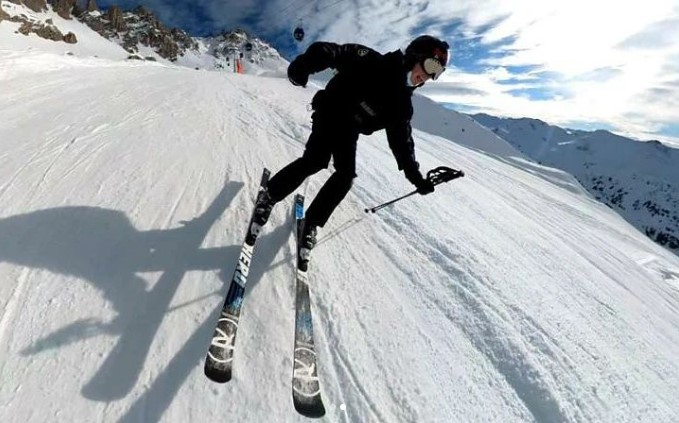
\includegraphics[width=\linewidth]{images/placeholder.jpg}
      &
      The cost of this vehicle could be larger than the other vehicles due to the aerodynamic body of the vehicle and the fact that there are two propellers. The dual prop design would also increase the amount of components in the drivetrain, increasing the cost.
      & 
      The finish is relatively clean for this vehicle, which improves the overall aesthetics. From analysis the streamlined body of the vehicle would add significant designing, to the project. 
      &  
      The drivetrain of this vehicle looks relatively modular, with the main structure being connected with bolts. The two-propeller system reduces the modularity of the vehicle.
      & 
      The two propellers would be able to be manufactured in tandem, but a significant amount of manufacturing would have to be completed to finish the vehicle.  
      &  
      The vehicle looks relatively stable, although the propeller looks relatively large in comparison to the vehicle which could cause oscillatory issues.
      &  
      The two-propeller system would generate a significant amount of thrust. 
      &  
      The vehicle is very complex with two propellers adding significant design for the drivetrain and the aerodynamics of the vehicle. 
      &  
      The vehicle has a lot of aerodynamic components that could be broken easily and would need to be replaced. Initially designing the vehicle for durability will therefore help improve the project, especially with us focussing on durability.
      \\ \hline
      
      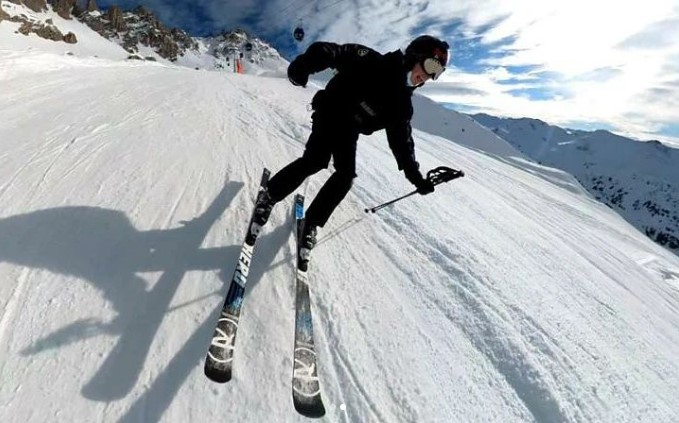
\includegraphics[width=\linewidth]{images/placeholder.jpg}
      &
      This vehicle looks very expensive due to the slick and streamlined nature of the body. The wheels are solid on this vehicle which would increase the expense of the vehicle significantly.
      &  
      The vehicle looks very aesthetically pleasing with the enclosed cockpit for the driver. The wheel covers add more to the design and make the vehicle look well engineered. 
      &  
      This vehicle doesn't look very complex. This is probably due to the fact that this vehicle is near the end of the design process and all components have been tested multiple times. 
      &  
      This vehicle will be difficult to manufacture. The aerodynamic body will have been made from a composite and the translucent window at the front will have been difficult to create. 
      &  
      This vehicle looks safe due to its enclosed cockpit design. The vehicle looks stable and there are obvious safety concerns that have been addressed on the vehicle. 
      &  
      This vehicle looks like it would performance well aerodynamically. The solid wheels will reduce the unpredictable nature of the wheels but will require additional suspension for the vehicle to run smoothly on the road. 
      &  
      The drivetrain system for this device looks like a shaft drive due to the thin pole supporting the vehicle. 
      & 
      As with the other vehicles, the outer casing will cause significant issues with durability, especially as composites can break with impacts. The wheels on this vehicle are an interesting prospect. 
      \\ \hline
      
      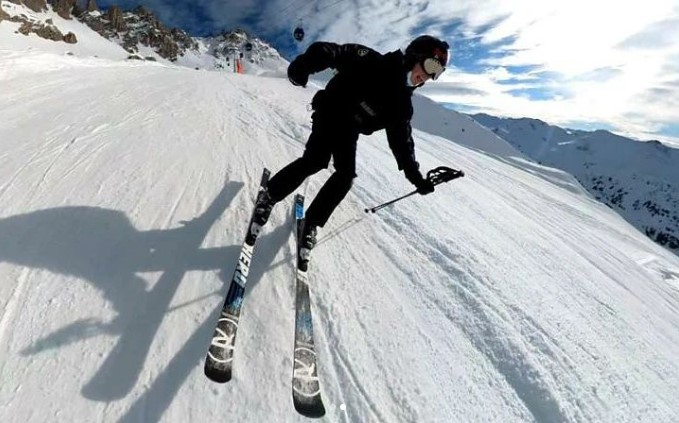
\includegraphics[width=\linewidth]{images/placeholder.jpg}
      &  
      This is the main vehicle that started the downwind faster than the wind theory. The propeller on this vehicle is large, therefore will cost a lot, adding to the already complex body.
      &  
      This vehicle looks relatively bulky but the significant aerodynamic components help improve the aerodynamics significantly. 
      &  
      As the vehicle has significant aerodynamic components that have been improved over a large amount of time, meaning most of the parts aren't replaceable. This vehicle isn't modular, and therefore takes a lot of work to maintain.
      &  
      Due to the complex components on this vehicle, this vehicle will be difficult to manufacture. On the whole the vehicle is complex to manufacture and is not a good vehicle to base our vehicle on.
      &  
      The YouTube video on this vehicle show significant oscillation when the propeller is moving quickly. The vehicle is not completely safe and has systems involved to stop the vehicle. Our vehicle is unmanned; therefore, these concerns will not be as significant. 
      &  
      This vehicle has shown incredible performance with good ability going upwind and downwind. The chain system on the vehicle provides significant tension for the propeller and spins and provides thrust at most speeds. 
      &  
      The vehicle is very complex in both aerodynamics and functionality. The vehicle can fold in half due to its size and need to be transported. The drivetrain of the vehicle although hidden is very complex and has been worked on for a long time.
      &  
      The vehicle is very large and components are state of the art for the vehicles, suggesting that they are not easily replaces. The vehicle frame is mechanical and therefore is prove to failure, and the structure is built from wood which with an impact could break 
      \\ \hline
    \end{tabular}
    \caption{Previous attempts at downwind-faster-than-the-wind vehicles}
    \label{tab:prevAttempts}
\end{table}
\twocolumn